\section{Synchronisation \label{sec:sync}}

Some programming techniques for parallel computers rely on efficient
synchronisation between some or all of the processes, so that they may operate
in unison. Synchronisation may be needed to detect termination, or to ensure
that all running processes have completed updates to a global state before
proceeding to the next stage of a computation.  

\emph{Barrier synchronisation} is a key operation in many parallel algorithms.
It is used to ensure that a set of processes enter a new phase of computation at
the same time. Any global communication such as a reduction (an operation such
as a sum or multiply performed over all elements of a distributed data set) or
scatter (to distribute data from one process to many processes) may imply the
use of a barrier.  Figure~\ref{fig:barrier} illustrates the operation of a
barrier. Processes may enter a barrier at any time, but may leave only once all
other processes have entered. 

\begin{figure}
\centering
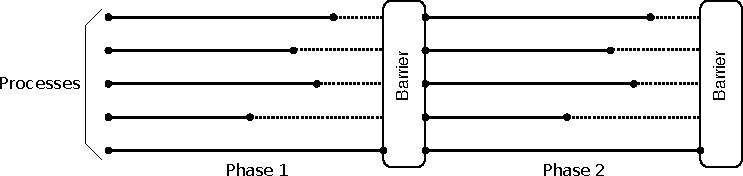
\includegraphics[scale=1]{../images/barrier.pdf}
\caption{Operation of a barrier. Some processes may complete a phase more
quickly than others, but the barrier ensures that all processes enter the next
phase synchronously.}
\label{fig:barrier}
\end{figure}

\emph{Clock synchronisation} is another form of synchronisation, necessary when
each node in a distributed system has access to its own clock, but no guarantees
can be made of the agreement with the clocks kept by other nodes.
Synchronisation can be performed globally so that there is a consensus on a
single time in the network.  Clock synchronisation is key to making accurate
measurements for message latencies, barrier synchronisations and traffic
patterns. 

\subsection{Barrier Synchronisation \label{sec:barrier}}

With a hypercube network, it is possible to perform a barrier synchronisation in
$O(\log N)$ communication steps, where $N$ is the number of nodes in the
network. In other network topologies such as meshes or irregular structures,
barrier synchronisation is typically implemented using tree structures which
incur a far higher cost.

The barrier synchronisation scheme for a hypercube works by synchronising with
neighbouring nodes, in each dimension in turn. To begin, each node exchanges a
single message with its neighbouring node. The first neighbour of node $i$ is $i
\oplus 1$, the second is $i \oplus 2$ and $i \oplus 2^d$ for dimension $d$.  In
the first exchange, all pairs of nodes connected in the first dimension become
synchronised with each other and we have $N/2$ synchronised pairs. In the second
exchange, nodes connected in second dimension become synchronised with those in
the first, producing $N/4$ synchronised groups. After $d$ iterations, all nodes
become synchronised in a single group. In this scheme, no node can leave the
barrier before all nodes have entered it. Algorithm \ref{alg:barrier} gives
pseudo-code that each node executes to perform a barrier synchronisation.

\begin{algorithm}
\caption{Barrier synchronisation executed by each node $m$ in the network.}
\label{alg:barrier}
\begin{algorithmic}
\FOR{$i=1$ to $d$}
\STATE Neighbour node $n = m \oplus 2^i$
\STATE Send message to $n$
\STATE Receive message from $n$
\ENDFOR
\end{algorithmic}
\end{algorithm}

This approach of iteratively exchanging messages in each dimension is a general
and useful communication pattern that can be applied to many other problems.
These include finding minimum and maximum values over the set of nodes and to
calculate the average of the values held by each node. In particular though,
global clock synchronisation can also be achieved in this way.

\subsection{Global Clock Synchronisation}

The aim of clock synchronisation is for each node to learn an offset value to
some reference clock in the network. This could be the average clock or that of
a specific node.

Synchronisation of clocks to a specific node for a hypercube works in the same
way as the barrier. Let $c_n$ denote the clock of node $n$. Initially, all pairs
of nodes connected in the first dimension exchange messages to determine the
offsets between their clocks. If synchronisation is based on $c_0$, then a
adjustments are applied in each exchange to the node with the largest identifier
value. If it is based on $c_{N-1}$, then adjustments are applied to the lowest. 

Using a similar inductive argument as the one used in \sect{barrier}, we can
show this will approach will result in global synchronisation. After the 
first exchange, each pair of nodes are synchronised and conceptually the network
contains $N/2$ different clocks. In the second phase, nodes exchange in the
second dimension, but \emph{include} the offset they learned in the first,
leaving $N/4$ different clocks. This continues until all nodes have learned their
offset from the reference clock. 

Pseudo-code for this process is given in algorithm \algo{clksync}.  The
functions $\clkSyncMaster$ and $\clkSyncSlave$ perform communication between
neighbours in a particular dimension to determine the difference $\Delta$,
between the two clocks such that $$\Delta = c_{n_u} - c_{n_v}.$$

\begin{algorithm}
\caption{Clock synchronisation pseudo-code for node $m$.}
\label{alg:clksync}

\begin{algorithmic}
\STATE $offset \gets 0$
\FOR{$i=1$ to $d$}
    \STATE Neighbour node $n = n \oplus 2^i$
    \IF{$m > n$}
        \STATE $\Delta \gets \clkSyncMaster$
        \STATE $offset \gets offset + \Delta$
    \ELSE
        \STATE $\clkSyncSlave$
    \ENDIF
\ENDFOR
\end{algorithmic}
\end{algorithm}

\subsubsection{Determining the Clock Offset Between Two Cores}

Accurately determining the value of $\Delta$ is key to the final synchronisation
between nodes.  This can be performed with two \emph{ping-pong} exchanges
between the \emph{master} and \emph{slave} processes. The master learns from
this two time values $t_0$ and $t_2$ recorded by the slave, and $t_1$, recorded
itself in the middle. The exchange is initialised by the slave node which sends
a message to the master.  When the master receives this, it replies. On
receiving this, the slave measures its time ($t_0$) and send this back to the
master. When the master receives it, it measures its own time ($t_1$), then
pings the slave again for another clock measurement ($t_2$) which is measured
and sent back in the same way. \fig{pingpong} illustrates this exchange. 

Using these values of $t_0$, $t_1$ and $t_2$, the following equations can then
be setup, where $h$ is a single hop time and $\epsilon$ is an error term.

\begin{eqnarray}
t_1 - t_0 & = & \Delta + h + \epsilon \label{eqn:xy}\\
t_2 - t_1 & = & -\Delta + h + \epsilon \label{eqn:zx}
\end{eqnarray}

\noindent
Subtracting \ref{eqn:zx} from \ref{eqn:xy} we can then obtain the value of
$\Delta$: $$\Delta = t_1 - t_0/2 - t_2/2.$$

\begin{figure}
\centering
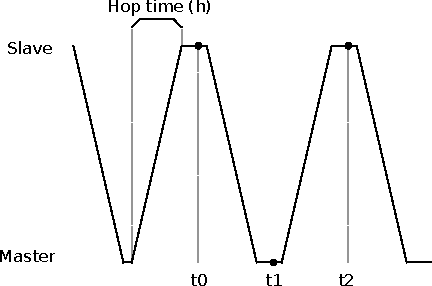
\includegraphics[scale=1]{../images/pingpong.pdf}
\caption{A diagram illustrating the exchanges made between the master and slave
nodes to obtain the values $t_0$, $t_1$ and $t_2$.}
\label{fig:pingpong}
\end{figure}

To reduce to a minimum any error in measurement, it is important for these
measurement operations to minimise the number of instructions and ensure the
exchanges are symmetric. As a result, the functions $\clkSyncMaster$ and
$\clkSyncSlave$ were implemented directly in assembly.

\subsubsection{Reducing Error in $\Delta$}

In practice, the true value of $\Delta$ cannot always be learned, and instead the
calculation may yield $\Delta + \epsilon$, where $\epsilon$ is some small error
value. This could be caused by non-determinism at the hardware level.  We know that the
calculation of $\Delta$ in a given dimension $d'$ should be the same for all of
the nodes that have already synchronised in the previous dimensions, of which
there will be $2^{d'-1}$. 

Using this invariant, we can reduce the effect of this error as we propagate an
offset through the cube by averaging over previous dimensions. Each node 
$m$ computes its $\Delta_m$ offset as the average over the other $\Delta$s
calculated in previous dimensions $0,\dots,d'-1$: 
$$\Delta_{m}(d') = \frac{1}{2^{d'-1}} \sum_ {n \in A(n,d')} \Delta_{n}$$ 
where 
$$A(m,d) = \left\{n \mid n=m\oplus 2^i \text{ for } 0 \leq i < d\right\}$$ 
is the set of neighbouring nodes of $m$ in dimensions $0, \dots,d-1$.
The calculation of the average at each node can be completed in $\log(2^{d-1}) =
d-1$ steps using the same dimension-ordered exchange procedure. 

\subsection{Timing a Barrier Synchronisation}

\subsubsection{Estimated Time}

A simple estimate of the time for a barrier synchronisation to complete can be
made by considering the single-hop times between cores.  As we can view the
XK-XMP-64 network as a $6$-dimensional hypercube, where the first two dimensions
are contained in-chip, the single hop time in-chip $h_{in}$ and off-chip
$h_{off}$ form this estimate. The time to run a barrier synchronisation (the
operation given in \algo{barrier}) is then $2 h_{in} + 4 h_{off}$. These times
are simple to measure and are presented in table \ref{tab:hoptimes}. Using them,
an estimate of 940ns for the barrier to complete can be made.

\begin{table}
\centering
\begin{tabular}{lc}
{\bf Core-to-core journey} & {\bf Time (ns)}\\
\hline
On-chip & 70\\
Off-chip (1 hop) & 200\\
Off-chip (2 hops) & 290\\
Off-chip (3 hops) & 390\\
Off-chip (4 hops) & 480\\
%%%% Check the last 2 values!!
\end{tabular}
\caption{Timings of core-to-core journeys, both on and off-chip. Note 4 is the
diameter of the hypercube; the maximum distance between any two nodes.}
\label{tab:hoptimes}
\end{table}

\subsubsection{Measured Time}

To make a precise measurement of the time taken for a barrier to complete, where
all nodes minimise their time in the barrier, i.e.\ that they enter at precisely
the same point in time (an assumption made by the estimate), it is
necessary to use globally synchronise clocks.

If nodes enter the barrier unsynchronised, some will enter before others,
completing exchanges in as many dimensions as they can but not completing until
all have entered. For those nodes entering late, they will complete much faster
then normal as messages will be waiting for them in one or more dimensions. In
one extreme, nodes $n_1$ to $n_{63}$ enter the barrier early, followed much
later by $n_0$. In this case, it takes $n_0$ just 280ns to complete the barrier
synchronisation.

For nodes to enter the barrier simultaneously, they must synchronise their
clocks against, for instance, node $n_0$ to obtain an offset to $c_{n_0}$ and
enter at a time in the future specified by $n_0$ adjusted by the offset to
$c_{n_0}$. If the synchronisation is perfect, then each node should spend
exactly the same amount of time in the barrier.

Using the above method, the elapsed time through the barrier was recorded for
each node. The results varied by a range of around 150ns each run, with minimum
and maximum times of approximately 930ns and 1100ns respectively, but with a
consistent average of 990ns, which is in-line with the estimate made by
considering single hop times.

Although the measurement error in the $\Delta$ term was reduced by averaging
over synchronised nodes, it still effects the synchronisation, evident in the
resulting times through the barrier. To ensure this error was not systematic in
the program code, the precise clock offsets were inspected by analysing signal
output from pins on the board. This revealed that offsets after synchronisation
between nodes $n_1$ to $n_{63}$ and $n_0$ varied between runs and hence could
not be caused by some bias in the measurement for example.

